\documentclass[oneside, german]{htwg-report}

% !TEX root = ../report.tex
% Use german umlaute
\usepackage{german,ngerman}
\usepackage[T1]{fontenc}
\usepackage[utf8]{inputenc}
\usepackage[ngerman]{babel}
\usepackage[autostyle=true,german=quotes]{csquotes}

%\usepackage[table]{xcolor}\usepackage{float}
%\usepackage{xcolor,colortbl}

\usepackage{epigraph}
\usepackage{float}
\usepackage{subfig}
\usepackage[backend=bibtex]{biblatex}

\addbibresource{report.bib}

\begin{document}

\pagenumbering{gobble}

%% 'reporttype' add background elements to the cover / front page
%% possible values are:
%% bachelor	--> B S C
%% master	--> M S C
%% other		--> none
\reporttype{master}

\reporttypetext{Teamprojekt}

\newcommand{\verfasserA}{Lukas Hornung}
\newcommand{\verfasserB}{Lukas Luschin}
\newcommand{\verfasserC}{Moritz Schmidt}
\newcommand{\verfasserD}{Timmo Waller-Ehrat}
\newcommand{\verfasserE}{}
\newcommand{\thema}{Mehrbildkamerasystem zur räumlichen Detektion von Modellhubschraubern}
\newcommand{\hoschschule}{Hochschule für Technik, Wirtschaft und Gestaltung}
\newcommand{\institut}{HTWG Konstanz, Institut für Optische Systeme}
\newcommand{\prueferA}{Prof. Dr. Georg Umlauf}
\newcommand{\prueferB}{Prof. Dr Matthias O. Franz}
\newcommand{\prueferC}{Dennis Griesser}


\title[Mehrbildkamerasystem zur räumlichen Detektion von Modellhubschraubern]{\thema}

\doclocation{Konstanz}
\docdate{01. April 2018}

\makecover[]
%          
%% Include an optional title page.
%% !TEX root = report.tex
\begin{titlepage}
\newgeometry{hscale=0.81,vscale=0.8}

\AddToShipoutPicture*{\BackgroundImgTitelPage}

\vspace*{\bigskipamount}


%% Print the title in htwg-teal.
{\makeatletter
\fboxsep=0pt
\colorbox{htwg-white}{\begin{minipage}[t]{145mm}
    \begin{center}
        %% Print Report Type Text
        \color{black}\Huge{\@report@typetext}
        \\
        %% Print Report Title
        \color{black}\Huge\textbf{\@title}
    \end{center}
\end{minipage}}
\makeatother}

\bigskip
\bigskip

{
\setlength{\parskip}{0.5cm}
\begin{center}
	\textbf{zur Erlangung des akademischen Grades}
	
	\textbf{\Large \type\ of Science (\typeshortcut. Sc.)}
	
	\textbf{an der}
	
	\textsf{\huge Hochschule Konstanz}\\
	{\small Technik, Wirtschaft und Gestaltung}
	
    \textsf{\Large Fakultät Informatik} \\
	Studiengang \studiengang
	
\end{center}
}

\bigskip
\bigskip
\bigskip

\begin{center}
	\begingroup
	\renewcommand*{\arraystretch}{1}
	\rowcolors{2}{white}{white}
	{\makeatletter
		\begin{tabular}{lll}
			\type kandidat: & \verfasser \\
							& \strasse \\
							& \wohnort \\ \\ \\ \\
	
			1. Prüfer: & \prueferA \\
			2. Prüfer: & \prueferB \\ \\ \\ \\
			
			Ausgabedatum: & \ausgabedatum \\
			Abgabedatum: & \abgabedatum
		\end{tabular}
		\makeatother}
	\endgroup
\end{center}


%% reset page margins
\newgeometry{hscale=0.7,vscale=0.8}
\end{titlepage}




% !TEX root = report.tex
\chapter*{Extended Abstract}

\begin{center}
	\begingroup
	\renewcommand*{\arraystretch}{1}
	\rowcolors{2}{white}{white}
	{\makeatletter	
		\begin{tabular}{p{3.2cm}p{9.6cm}}
			Thema: & \thema \\
			& \\
			Teammitglieder: & \verfasserA, \verfasserB, 
			\verfasserC, \verfasserD\\
			& \\
			Betreuer: & \hoschschule \newline \institut \newline \prueferA, \prueferB \\
			& \\
		\end{tabular}
		
		\makeatother}
	\endgroup
\end{center}

\bigskip

\noindent
Unser Projekt behandelt das r"aumliche Detektieren eines Modellhubschraubers. Die Detektion soll unter Laborbedingungen, das hei"st, der Helikopter befindet sich vor einer wei"sen Wand, stattfinden. Mittels der Detektion soll auf einem Bild angezeigt werden, wo sich der Mittelpunkt des Helikopters befindet. Auch die Tiefe (Entfernung zur Kamera) des Helikopters soll ermittelt werden. F"ur diese Detektion sollen zwei oder mehr Kameras verwendet werden. Bei diesen handelt es sich um HIERKAMERAEINF"UGEN, die mit dem Computer "uber ein FireWire-Kabel verbunden sind.\newline

\begin{figure}[H]
	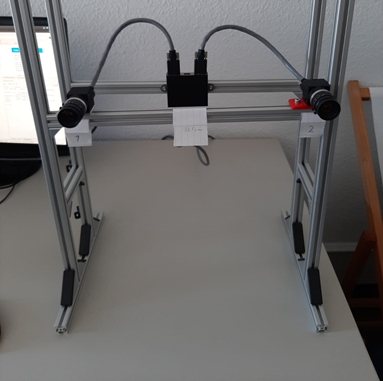
\includegraphics[scale=1.0]{bilder/camerasystem}
	\caption[Kamera-System]{Kamera-System}
\end{figure}

\noindent Das Projekt wurde erfolgreich umgesetzt.
Mittels zwei Kameras, die auf einer geraden Linie angebracht sind, kann der Mittelpunkt des Helikopters und dessen Abstand zur Kamera ermittelt werden.\newline
Unser Programm kalibriert als erstes die Kameras einzeln und anschlie"send zu einander. Das Kalibrieren erfolgt "uber ein Schachbrett-Muster. Sind die Kameras zueinander kalibriert, kann mittels eines Feature-Detektors eine Punktewolke des Helikopters generiert und der Mittelpunkt berechnet werden.

\begin{figure}%
	\centering
	\subfloat[Kamera-Kalibrierung]{{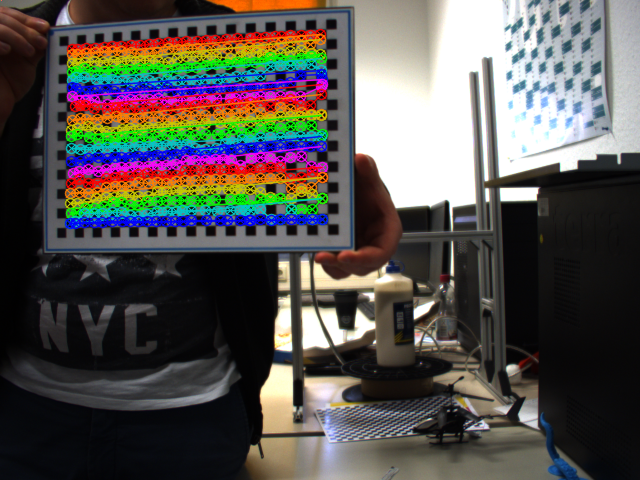
\includegraphics[width=6cm]{bilder/calibration} }}%
	\qquad
	\subfloat[Helikopter-Punktewolke]{{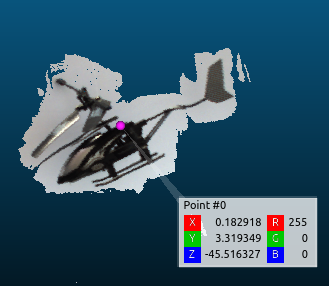
\includegraphics[width=6cm]{bilder/helicloud} }}%
	\caption{Kamera-Kalibrierung und Punktewolke}%
	\label{fig:example}%
\end{figure}
\noindent Eine m"ogliche Erweiterung des Projekts w"are das Kalibrieren von zwei Stereo-Systemen zu einander, um eine noch h"ohere Genauigkeit zu erlangen. Dies wurde versucht umzusetzen, ist allerdings gescheitert.


% !TEX root = report.tex
\chapter*{Abstract}
Ziel des Projekts war das r"aumliche Detektieren eines Modellhubschraubers. Die Detektion soll unter Laborbedingungen stattfinden. Das hei"st, der Helikopter befindet sich vor einer wei"sen Wand.
Zur Lokalisierung des Helikopters im Raum soll zun"achst eine 3D-Punktewolke der Szene generiert und daraus mit Hilfe des Clustering-Algorithmus k-Means die Position des Helikopters bestimmt werden. Auch die Tiefe (Entfernung zur Kamera) des Helikopters soll ermittelt werden. Die Detektion soll mit Hilfe von zwei oder mehr Kameras des Herstellers Point Grey, die "uber eine FireWire-Schnittstelle mit einem Computer verbunden sind, stattfinden.

\tableofcontents
\newpage
\chapter{Einleitung}
\label{cha:einleitung}

\section{Aufgabenstellung und Zielsetzung}
\label {sec:aufgabenstellungzielsetzung}

Im Rahmen dieses Teamprojekts stand die Entwicklung eines Mehrbildkamerasystems zur r"aumlichen Detektion eines Modellhubschraubers. Dies beinhaltet sowohl das Erkennen des Helikopters, als auch die Abstandsmessung von diesem. Dies sollte mit Hilfe von Bilderverarbeitungs- und Machine Learning-Techniken, sowie der Verwendung von zwei oder mehr Kameras umgesetzt werden.\newline
Die Lernziele umfassten das Erlernen des Umgangs mit Kameras f"ur die industrielle Bildverarbeitung, sowie ein Verst"andnis f"ur die Grundlagen industrieller Signalverarbeitung zu schaffen. Zudem sollten grundlegende KI-Verfahren erlernt werden.

\newpage

\section{Motivation}
\label {sec:motivation}

\setlength\epigraphwidth{15cm}
\setlength\epigraphrule{0pt}

\epigraph{\textit{\glqq Computer vision, or the ability of artificially intelligent systems to see like humans, has been a subject of increasing interest and rigorous research for decades now.\grqq{}}}{--- \textup{}Naveen Joshi\cite{NJ}\\}

\noindent Das maschinelle Sehen gewinnt in den letzten Jahren immer mehr an Popularit"at. Sei es in der Forschung oder z.B. in der Spieleentwicklung f"ur Augmented Reality. Durch die steigende Relevanz in der Praxis wurde auch unser Interesse f"ur dieses Themengebiet geweckt. Es ist spannend zu verstehen, wie komplex die Dinge, die f"ur uns Menschen selbstverst"andlich erscheinen, wie zum Beispiel das r"aumliche Sehen, eigentlich sind.
Ein weiterer Anreiz f"ur das Projekt waren die verschiedenen angewandten Technologien. Wir alle interessieren uns sehr f"ur das Programmieren. Viel Erfahrung in der Programmiersprache Python hatte aber anfangs keines der Teammitglieder. Somit war das Erlernen dieser Sprache eine weitere Motivation.\newline
Auch die zum Gro"steil verwendete und weit verbreitete Bibliothek f"ur Computer Vision-Anwendungen in Python ''OpenCV'' hat das Interesse an dem Projekt geweckt.

\section{Aufbau}
\label {sec:aufbau}
Die Ausarbeitung des Teamprojekts besteht aus drei Teilen.\newline
Anfangs wird kurz auf die angewandten Technologien eingegangen.
Anschlie"send wird die eigentliche Umsetzung und das Vorgehen erl"autert. Zuletzt wird auf die aufgetretenen Probleme eingegangen und ein Fazit gezogen.

\input{Technologien}
\chapter{Bildverarbeitung und Umsetzung}
\label{cha:verarbeitungumsetzung}

\section{Kalibrierung}
\label{sec:kalibrierung}

F"ur eine Messung, bei der der Fehler minimiert werden soll, ist das Kalibrieren der Kameras unumg"anglich. Durch die Linse einer Kamera entsteht eine tonnenf"ormige Verzeichnung. Diese Fehler sind meist so klein, dass sie vom menschlichen Auge nicht erfasst werden k"onnen \cite{VZ} \cite{VZ1}. Durch die Kalibrierung der Kamera k"onnen diese kompensiert werden.\newline

\begin{figure}[H]
	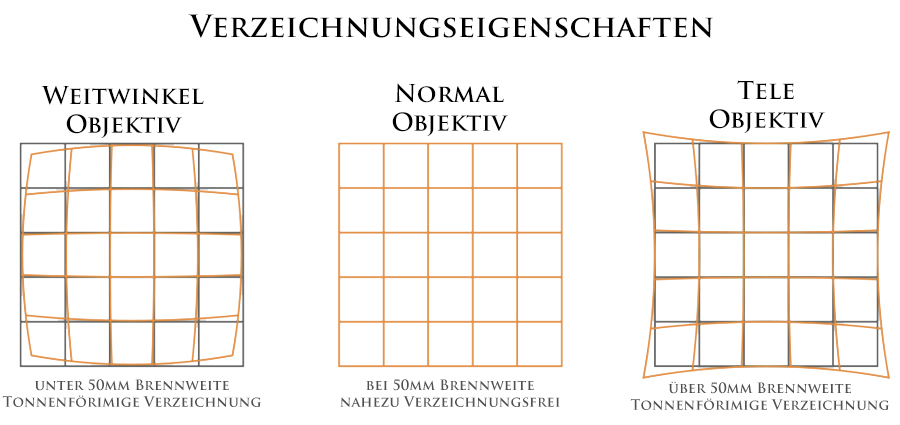
\includegraphics[scale=0.45]{bilder/verzeichnung}
	\caption[Verzeichnung]{Verzeichnung}
	\small Quelle: \url{http://www.fotokurs-bremen.de/wp-content/uploads/2016/11/Objektiv-Verzeichnung.jpg}
\end{figure}

\noindent Durch die Kamerakalibrierung werden folgende Parameter bestimmt:

\begin{description}
	\item[Intrinsische Parameter]
	Bezeichnen die Abbildung von 3D-Punkten im Kamerakoordinatensystem auf den 2D-Sensor der Kamera. Es sind Informationen der Kamera selbst, die unabh"angig davon sind, wo sich die Kamera befindet und wie diese ausgerichtet ist \cite{Intr}.
	
	\item[Extrinsische Parameter]
	Die r"aumliche Lage und Orientierung der Kamera zu einem Referenzkoordinatensystem, d.h. die Rotation und Translation \cite{cal} \cite{extr}.
\end{description}

\noindent Da es ich bei dem System um ein Stereokamera-System handelt, ist die Kalibrierung von diesem etwas komplizierter.\newline
Zuerst m"ussen die Kameras gesondert kalibriert werden. Dies wird mit der Funktion \textit{calibrateCamera} von OpenCV durchgef"uhrt. F"ur die Kalibrierung wird ein Schachbrett-Muster verwendet. Wichtig ist, dass bei der Kalibrierung beide Kameras dasselbe Bild verwenden. F"ur die Erkennung des Schachbretts wird die OpenCV-Funktion \textit{findChessboardCorners} verwendet. Diese liefert die Objekt- und Bild-Punkte der Aufnahme. Bei den Objekt-Punkten handelt es sich um die 3D-Punkte des Bildes, bei den Bild-Punkten um die 2D-Punkte \cite{OcvD}.

\begin{figure}[H]
	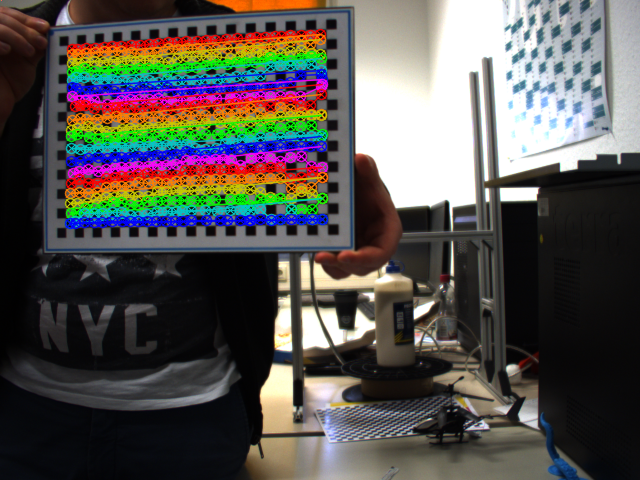
\includegraphics[scale=0.4]{bilder/calibration}
	\caption[Kalibrierung]{Kalibrierung}
\end{figure}

\noindent F"ur eine m"oglichst genaue Kalibrierung werden 50 Bilder verwendet. Anhand dieser wird jede Kamera mittels \textit{calibrateCamera} kalibriert.\newline
Die Funktion liefert die intrinsisches Parameter in Form von einer $3x3$ Kamera-Matrix

\begin{figure}[H]
	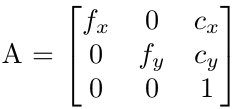
\includegraphics[scale=0.75]{bilder/matrix}
\end{figure}

\newpage

\noindent Wobei $f_{x}$ und $f_{y}$ die Brennweite in Pixeln und $c_{x}$ $c_{y}$ ein Hauptpunkt, der normalerweise in der Bildmitte liegt, ist.

\noindent Die Ergebnisse dieses Vorgangs werden auf dem Computer gespeichert, sodass dieser nicht wiederholt werden muss. Anschlie"send wird das Ergebnis der Kalibrierungen an die OpenCV-Funktion \textit{stereoCalibrate} "ubergeben.\newline
Mit Hilfe der Stereo-Kalibrierung kann der Zusammenhang zwischen den Kameras ermittelt werden: Es werden von dem Bezugsbild, welches zum Ursprung des Koordinatensystems wird, die Objekt-Punkte verwendet. Von beiden Kamerasystem werden die Bild-Punkte, die jeweiligen Kameramatrizen und die Verzeichnungskoeffizienten verwenden.

\section{Tiefeninformationen}
\label{sec:tiefeninformationen}

\noindent Das Verwenden des Stereo-Kameras ist relevant f"ur die Berechnung von Tiefeninformationen. Da die Information der Tiefe nicht in einem einzigen Bild ermittelt werden kann, wird eine zweite Kamera hinzugef"ugt. Diese ist im Raum verschoben, fotografiert aber zum gr"o"sten Teil die gleiche Szene.

\begin{figure}%
	\centering
	\subfloat[Stereosystem]{{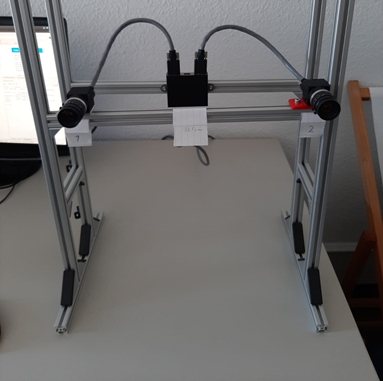
\includegraphics[width=6cm]{bilder/camerasystem} }}%
	\qquad
	\subfloat[Szenenaufnahme]{{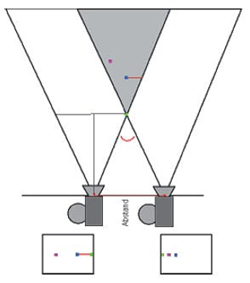
\includegraphics[width=6cm]{bilder/szene} }}%
	\caption{Stereo-System}%
	\small Quelle: \url{https://me.efi.th-nuernberg.de/interaktion/index.php5/Bearbeitung_und_Gewinnung_von_Tiefeninformation_durch_die_Kopplung_zweier_Kameras}
	\label{fig:stereo}%
\end{figure}

\noindent in \ref{fig:stereo}, im rechten Bild, ist in grau der Ausschnitt zu sehen, der von beiden Kameras erfasst wird. Das Bild daneben zeigt den Versuchsaufbau: zwei Kameras, die horizontal verschoben sind. Somit erhalten wir den Normalfall, der wie folgt beschrieben wird: \textit{Das achsparallele Stereosystem zeichnet sich durch zwei Kameras aus, die nur horizontal verschoben und deren Koordinatensysteme nicht gegeneinander verdreht sind \cite{Tu}.}\newline
\noindent Nun ist es m"oglich, "uber die Ungleichheiten des "uberlappenden Bildbereichs Tiefeninformationen zu ermitteln. Diese wird mit Hilfe der Disparit"at berechnet.\newline
Der horizontale Abstand, des gleichen Merkmals in beiden Bildern nennt man Disparit"at. \textit{Die Disparität ist umgekehrt proportional zur Tiefe. \cite{Tu}.}\newline
Durch die achsparallele Anordnung der Kameras, die nicht gegeneinander verdreht ist, kann die Z-Koordinate "uber die bekannten Kameraparameter, die Brennweite $f$ der Kameras und der Basisl"ange $B$ (Translation der Kameras zueinander), sowie die Disparit"at $D$ bestimmt werden. $D$ wird wie in \ref{fig:base} schematisch dargestellt, durch die Bildpunktverschiebung der Beiden Punkte $x$ un $x'$ berechnet. Der Z-Achsenwert berechnet sich mit der Formel $Z=\frac{f*B}{x-x'}$
 
 \begin{figure}[H]
 	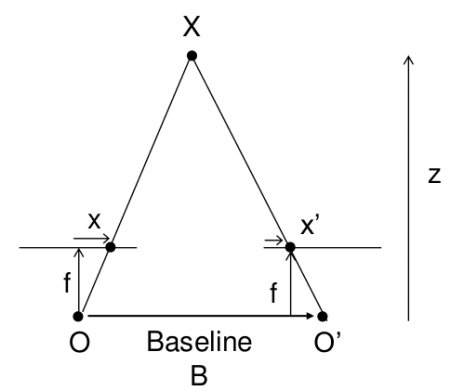
\includegraphics[scale=1.0]{bilder/tiefenberechnung}
 	\caption[Tiefenberechnung]{Tiefenberechnung}
 	\small Quelle: \url{https://opencv-python-tutroals.readthedocs.io/en/latest/py_tutorials/py_calib3d/py_depthmap/py_depthmap.html}
 	\label{fig:base}%
 \end{figure}
 
\newpage

Diese Funktion kalibriert die beiden Kameras zueinander. Dies geschieht mit Hilfe der vorher berechneten Kameramatrizen, Verzeichnungen und der Objekt- und Bild-Punkte.\newline 
Die wichtigsten Ergebnisse der Stereo-Kalibrierung sind die Rotation und die Translation der beiden Kameras zueinander.

\subsection{Fehler"uberpr"ufung}
\label{sec:fehlertest}

\section{Tiefeninformationen}
\label{sec:tiefeninformationen}

Um Tiefeninformationen aus zwei Bildern zu gewinnen, m"ussen diese zuerst rektifiziert und entzerrt werden. 

\chapter{Probleme}
\label{cha:probleme}

Trotz dem Erfolgreichen lokalisieren unseres Helikopters, hatten wir einige langwierigen Schwierigkeiten, die auch nicht bis zur Beendigung des Projektes gelöst wurden. Das Hauptproblem, mit dem wir nicht gerechnet hatten, war die Kalibrierung und die vielen Folgeprobleme, die sich daraus entwickelten. Nach dem Arbeitspaket Kalibrierung, in dem wir uns eingelesen, selbst kalibriert haben und unsere Methode mit den Methoden von OpenCV verglichen haben, sind wir davon ausgegangen das Thema sei abgeschlossen. Aber eine plausible Validierung aus den Daten war für uns nicht möglich. Die erhaltenen Werte konnten nicht eingeordnet werden, ob diese gut oder schlecht sind. Zwar versuchten wir immer wieder mit neuen Messungen dies zu bestätigen, aber ein konsistenter Beleg, dass unsere Kalibrierung exakt ist, war nicht möglich. So dachten wir oft wir hätten dieses Thema erfolgreich beendet, aber bei Fehlschlägen in weiterführenden Themen, wie große Unstimmigkeiten in den Resultaten, konnte durch eine exaktere Kalibrierung bessere Ergebnisse erreicht werden. Die Ergebnisse schwankten auch sehr stark, wie die Lichteinstrahlung zu Zeiten der Messung im Labor war. So war es oft am besten abends Aufnahmen zu machen, da kein direktes Licht auf unseren Versuchsaufbau fiel. Trotz des abhängen des Fensters, war es nicht möglich dieses Schwanken zu eliminieren. Dies führte auch bei Erfolgen schnell zu einer Demotivation weiter zu machen, da eine andere Fehlerquelle nicht auszuschließen war. Es konnte auch kein Arbeitspaket wirklich beendet werden, da es nicht m"oglich war, dieses als erfolgreich abgeschlossen zu deklarieren.

\noindent Wir haben mit der Kalibrierung von zwei Kameras zueinander gestartet, was viel Zeit in Anspruch genommen hat. Als wir unseren Aufbau um ein weiteres Kamerasystem erweitert haben, war es nicht mehr möglich Bilder aufzunehmen. Dieses Problem konnte durch eine Reduzierung der Bildgröße behoben werden. Es resultierte, dass alles neu kalibriert werden musste.\newline

\noindent Des Weiteren war es uns oft nicht möglich aus der OpenCV Dokumentation die richtigen Schlüsse zu ziehen, da sie lückenhaft und teilweise veraltet war. Daraus resultierten Fehler, welche laut der Dokumentation nicht passieren sollten.\newline

\noindent F"ur das Ansteuern der Kameras wurde die Bibliothek ''PyCapture2'' verwendet. Diese hatte aber keine vernünftige Dokumentation, was die Anbinden der Bibliothek deutlich erschwert hat.\newline

\noindent Die f"ur die Entwicklung verwendete IDE Spyder hat sehr begrenzte Debug-M"oglichkeiten. So ist es zum Beispiel nicht m"oglich, sich im Debug-Modus gro"se Matrizen anzuzeigen, was die Fehlersuche oftmals schwieriger gestaltet hat.


\printbibliography
\listoffigures

\end{document}

